\chapter{Background} %better name?
\label{ch2}

In Chapter~\ref{ch1}, the background and reason for this project was briefly explained. Previous work on similar topics as well as the methods used was also discussed and a brief summary of the rest of the text was provided. In this chapter, some basic concepts for MMORPGs are described and parts of the architecture used behind the scenes of these games are discussed. Proceeding from MMORPGs the focus shifts to WoW, going into more detail as to how WoW works and familiarising the reader with some of the game terms and concepts.

Finally ArcEmu is discussed, explaining what it is, how it came about and why it was used in this project. This chapter should give the reader enough background to fully understand terms, concepts and explanations discussed further on in this text.

\section{General MMORPG mechanics} 
\label{mechanics}
%\subsection{History}
%The history of MMOGs is longer than most people are aware of. MMOGs as we know them today originated from a game called Multi-User Dungeons(MUD), which was a text-based role-playing game (RPG) that ran on the Essex University network from 1978 ~\cite{mmoghist, mud}. After MUD, Air Warrior was a large milestone for MMOGs when it was released in 1987. It was the first graphical MMOG and was available on GEnie, a new online service at the time ~\cite{airwarrior}. 

%The first MMOG to be played on the commercial Internet was a game called Meridian 59, which was released in 1996. This game allowed a large number of players to play in a single, persistent world that continued to exist when players logged out. Having a persistent and continuing world and allowing thousands of players to log into that world are both considered to be important characteristics to MMOGs today ~\cite{mmoghist}. The MMOG genre of games continued to grow in popularity, and different categories of MMOGs became available over time, the most popular being MMORPGs ~\cite{exploitingbook}.

%\subsection{MMORPGs}

As the name suggests, MMORPGs are role-playing games where thousands of players can log into a virtual game world to play together. Although there are many different MMORPGs available, most of them have a few characteristics in common. These similarities include the following: %having a customizable character or avatar, a way to improve your character as you progress, in-game social interaction and culture, and system architecture. 

\begin{enumerate}
	\item Having a customizable character or avatar.
	\item Having a way to improve your character as you progress.
	\item In-game social interaction and culture.
	\item System architecture.
\end{enumerate}


The system architecture refers to the technical functioning of MMORPGs, of which a simplified version is depicted in figure \ref{architecture}.%insert figure here.

\begin{figure}[htbp]
\centering
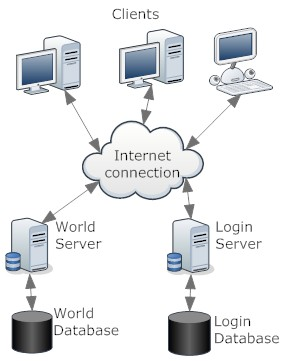
\includegraphics[scale = 0.5]{architecture.jpg}
\caption{Standard MMORPG system architecture}
\label{architecture}
\end{figure}

As can be seen from figure~\ref{architecture}, an MMORPG game has clients that log into the main server by first accessing the login server with their login details. The login server then verifies the login details by sending a query to the login database, and comparing the details. If the username and password are correct, the client gets logged into the world server, where the gameplay takes place~\cite{mmorpgarch}. The client is the software installed on your computer that you use to play the game. It is responsible to take all the input received from the user and the server, and to change the game display accordingly. The data sent and received from the server also has to be encoded and decoded by the client for safety reasons. Most of the data of MMORPG's is stored on your computer, because the Internet is still to slow to send all that data during gameplay. This means that the graphics that make up the game world, all the sounds and even how the monsters look are all stored on your computer in files and databases, and are processed by the client during gameplay.

The server still has a lot of things to compute however, especially considering the amount of players it services. Here is a list of some of the most common computations and functions the server does and sends back to the clients~\cite{serverclient}:

\begin{itemize}
    \item The position of your character in relation to monsters, players and non-playing characters (NPCs)
	\item Whether the monster that the player wants to attack is within range
	\item Whether your player is being attacked
	\item If your attacks are successful
	\item The amount of damage or healing given and received
	\item What loot will drop when a monster is killed
	\item The server also retrieves the skills, spells and items of your character from the database, and regularly saves your data in the database.
\end{itemize}

This type of server-client architecture is common in most of the more popular MMORPGs, and it works efficiently.  %The popularity of some common MMORPGs are shown in Figure \ref{popularity}.
%
%\begin{figure}[htbp]
%\centering
%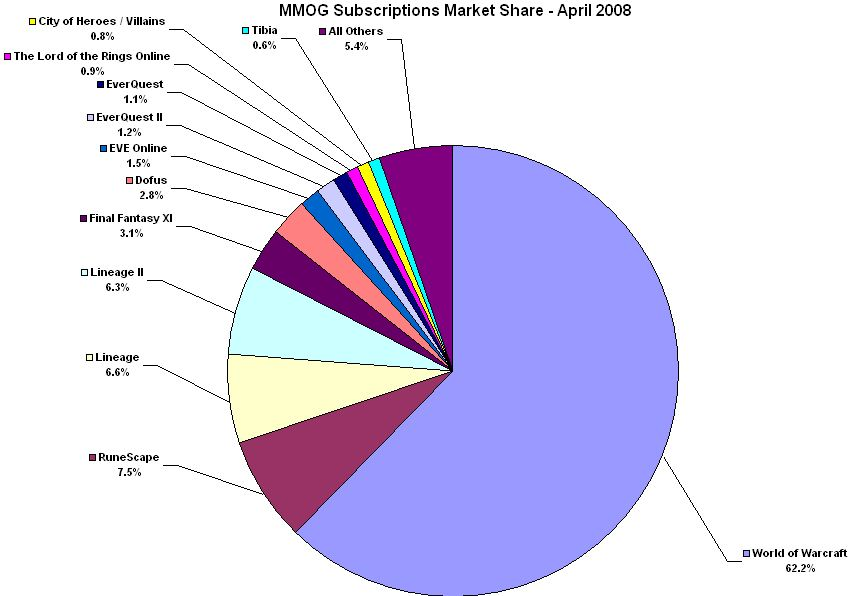
\includegraphics[scale = 0.65]{popularity.jpg}	%http://www.mmogchart.com/Chart7.html how to ref?
%\caption{The popularity of a few MMORPGs measured in percentage of subscribers}
%\label{popularity}
%\end{figure}
WoW is by far the most popular MMORPG in the world, which is why it was chosen for this project~\cite{subscription}.
%As can be seen in figure \ref{popularity}, WoW is by far the most popular MMORPG, which is why it was chosen for this project.


%Explain the basics of MMORPG's and the server-client architecture with the underlying database. Mention that WoW is the most subscribed to MMORPG which is why it was chosen to be the target MMORPG to track players. Mention research done on MMORPGs and why its important. Remember client side states being a security threat mentioned in book on how to exploit.

%\section{A Short History of WoW}

%Give a brief overview of when WoW was created and the previous Warcraft games that inspired it. Mention the expansion packs released, how the client is the same for all subscribers, disregarding whether they have the expansion or not, and also mention how the client is constantly updated, changing key features of how the game works (a few examples could be mentioned). 

%Also talk about where the game might be headed, mentioning growth in the game, how subscribers have now lessened and the possible reasons for it as well as how it will probably become more when new content and expansions are introduced. Remember the plague.

\section{World of Warcaft} %better name?

World of Warcraft is a fantasy role playing game created by Blizzard, set in the fantasy world of Azeroth. Blizzard created the world of Azeroth long before WoW was released, and used it in all of its previous strategy games in the Warcraft series. After Warcraft 3 was released, Blizzard decided to turn the franchise into an MMORPG.

\subsection{Starting the game}
When a user first plays WoW a long process of learning is started since it is a complex game. The first step for a new player is to choose a hero which will be their character or avatar in-game. There are two main sides in WoW, the Alliance and the Horde. Each side has different characters of different races that the user can choose from. These include races such as Humans, Dwarves, Orcs and so forth.
Each race has different classes of characters too, such as a Mage, Priest, Warrior and so forth. The user must create a character by choosing a race, class and name before entering the game world.

%Because there are so many people that play WoW, Blizzard split the game up into different Realms. Each Realm is an exact same copy of the game world, and is only there to split users up into more manageable groups of players. Each Realm has different servers and databases, and characters have to stay in the Realm in which they were created. Realms are also split up into different experience levels. There are different Realms for beginner, moderate and experienced players. 

Once the game is started, there are several non-player characters (NPCs) around, controlled by the server, that gives quests to the local character. Each quest has several rewards for the character, such as experience, items and gold. There are also NPCs that buy and sell items, or repairs items, or teaches your character new skills.

Users interact with the game world by using their keyboard or mouse for movement, and the user interface(UI) to select targets and other objects. %The UI is also useful for providing shortcuts to different spells and other attacks that can be used on monsters in the game.
 Figure~\ref{ui} shows a screenshot where a Warlock is in battle with a monster. The UI can also be seen, with lots of spells being displayed at the bottom of the screen for easy access. The health, mana and names of both the local character and its target is shown in the top left corner of the screen. %Characters consume either mana or rage when using certain abilities, depending on their class.

\begin{figure}[htbp]
\centering
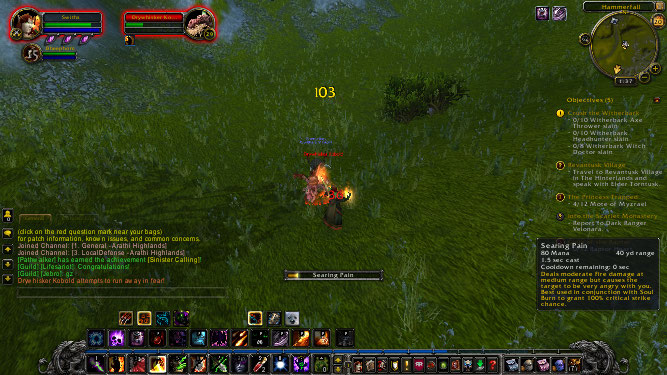
\includegraphics[scale = 0.65]{wowscreen.jpg}	
\caption{A screenshot showing the user interface of WoW}
\label{ui}
\end{figure}

Monsters in WoW are called ``critters'' officially, but are referred to by all the players as ``mobs''. %The mobs in WoW all have a level that indicates how powerful they are. 
%Your character also has a level, and is usually able to kill mobs of the same level and lower easily.
 Killing mobs and completing quests give experience to your character. Your character has an experience bar that measures the amount of experience it has. When this bar is full, the character levels up and the bar is emptied. Each level requires more experience to fill the bar up than the previous level. The top level in WoW is level 85, which can take several weeks of playing to reach.

When a mob is killed, it usually drops items and gold, which is called loot in the game. Items can enhance skills of your character, such as its attack and defense skills. There are many items in WoW, and a lot of motivation to get because they help your character to level up quicker. Items can also be sold for gold, and the gold can be used to buy items from other players or NPCs. 

The game also has professions, which are special skill sets that your character can learn. These include professions such as mining and engineering. Each profession has different advantages to the character, and only two can be learned at a time. 

The game world has large open areas, forests, caves and so forth where mobs are usually found. These are unfriendly areas where your character is in constant danger of being attacked. There are also more friendly areas such as towns where the NPCs that give quests and buy and sell items are found. The largest of these areas are called capital cities, where hundreds of NPCs that teach different skills and sell different things can be found. Capital cities are densely populated and many human players can be found there as they all look for items to buy and so forth.

The most human traffic in a capital city is in its bank and auction house. Players must keep all the items they pick up in their backpack and in satchels. This space is expended quickly when a lot of valuable items are found. The game provides banks in capital cities as extra storage place for players. The most valuable items of a player are stored in banks for future use or to sell them. If a player has a valuable item that is no longer of use to his character, the player can either sell the item to an NPC or at an auction house.

Auction houses list items that players want to sell and for which price. Other players then buy the items that interest them, and the money is transferred to the owner of the item. More gold can be made from selling items in auction houses than from selling them to NPCs. This causes a lot of traffic between auction houses and banks, which are usually located close to each other in capital cities, as players go get their rare items in the bank and then go to the auction house to list them. All this traffic makes capital cities a good place to track player movements to test the software.

All of these different skills, spells, professions and items that belong to your character has to be stored by the server in a database. This data changes frequently during game play and must be sent to and from the database through different queries constantly. It is of interest how much the data of a single player changes during a gaming session, and especially so of multiple players. This will be looked into further in chapter~\ref{database}.

%\subsection{Game Types}
%
%There are a few different game type categories in WoW, each providing a unique gaming experience. The type of player traffic found in each game type is considerably different. The game types where player movement data will be captured as test cases are briefly described here:
%
%\begin{itemize}
%	\item Open-World PvP/PvE
%	
%	This is the first type of gameplay a new player will be subjected to. PvE stands for player versus environment, and PvP for player versus player. The only difference between the two is that in PvP players from different factions can attack each other at any time, while in PvE both players first have to agree to fight before a battle can commence. This gameplay mode is mostly about completing quests, with some mobs being hard enough to require a team of players to defeat. For the most part this game type can be played alone if the user wants to.
%	
%	\item Dungeons
%	
%	The mobs in dungeons are smarter and stronger than the ones that can be found in the open world. A dungeon is a separate instance of WoW that can not be reached by walking around in the game world. A group of five players enter a dungeon together as a team and they work together to defeat the more difficult mobs. These mobs drop rare items and give more experience than normal mobs when killed, providing good motivation for players to enter dungeons.
%	
%%	\item Raids
%%	
%%	Raids are similar to dungeons, but with even stronger mobs which are harder to kill. The areas are bigger than dungeons, and groups of 10 to 25 players usually team up to complete a raid. The most powerful and valuable items can be found in raids.
%%	
%%	\item Battlegrounds
%%	
%%	Battlegrounds are PvP	battlefields , where players of opposite factions are constantly fighting over strategic targets. These include things such as keeping an area under your factions control, capturing the opposing faction flag, or killing the commander of the opposing faction. Some battlegrounds can have hundreds of different players participate in a single battle. Powerful items can also be gained here.
%%	
%%	\item The Arena
%%	
%%	In The Arena, organised teams of 2, 3 or 5 players of opposite factions commence in battle. The objective is to defeat all the members of the opposing faction. Unique items are also found in The Arena.
%	
%\end{itemize}



%
%\subsection{Team Play}
%%The different game types offer lots of motivation for players to team up in WoW.
%Playing a game as part of a team usually has the result that the team works closely together. Since the movement data of players in WoW is of interest, team play is important to keep in mind when tracking player movements.
%There are several different types of teams that can be created in WoW. A user can invite any other player from the same faction  %and in the same Realm 
%to join his group. 
%A group of up to 5 players is called a party, while a group between 10 and 25 players is a raid.
%If you enjoy playing with a certain player, you can add that player to your friend list and be notified when that player comes online, to make playing together again in future easier. 
%
%Another type of group that exists in WoW is called a guild. Parties and raids are only temporary groups, but guilds are permanent groups of players. There are many benefits of joining a guild, such as gaining access to the guild bank and having easier access to other players to form parties or raids.
%
%All of this team play in WoW is one of the reasons that it is thought that players move together often in the game.  % It is especially expected in areas such as battlegrounds and raids. 
%Tracking software can be used to confirm this suspected behaviour and to generate general player movement models. 


\subsection{Factors that influence tracking} 

There are a few factors that need to be kept in consideration when tracking players in WoW. The different levels that players are at give them access to different methods of traveling around. At level 20 a character can learn the skill of Riding, and a mount can be bought. This increases the movement speed of a player with 60 percent. At level 40 the skill can be increased and a faster mount can be bought that increases movement speed up to 100 percent. 

At later levels flying mounts can be bought, and these also get upgraded so that a character of level 85 can have a flying mount that increases movement speed by 392 percent if the proper aura is activated~\cite{mount}.

If tracking data shows what appears to be a player moving through buildings at high speed then it is very likely a player on a flying mount, flying over the buildings. This high movement speed also makes the server send less data to you since it can compute that you will not be able to see the player very long. Figure~\ref{flymount} shows a character on a flying mount, flying over trees into the city of Stormwind.

\begin{figure}[htbp]
\centering
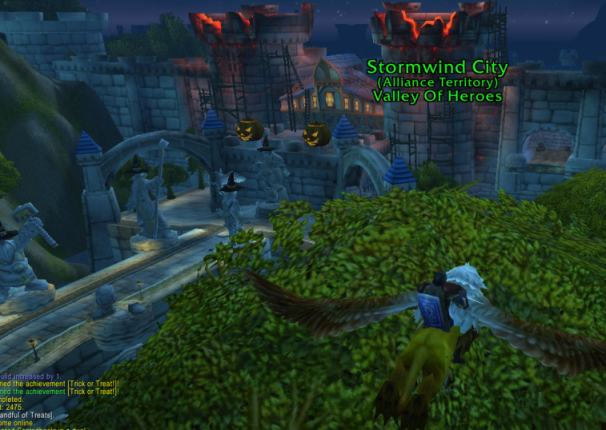
\includegraphics[scale = 0.65]{flystormwind1.png}	
\caption{A player on a flying mount, flying into Stormwind}
\label{flymount}
\end{figure}


The server tries to send your character relevant data and to minimize the irrelevant data. If players are within visual range of your character, but behind a big mountain then it is likely that the server could decide not to send the location of the other player to your client.

When entering WoW, your character suddenly appears in the world without coming from anywhere specific. This could result in tracking data where players appear to come out of nowhere. A player can also log out at any time, which would cause the player to disappear in the tracking data.

Some players in WoW have the ability to cloak themselves, rendering them invisible to other players. The server does not send the location of invisible players to your client, so when a player goes invisible the tracking data will stop without explanation. 

One big problem with tracking players in WoW from South Africa is the Internet. South Africa is behind the rest of the world when it comes to Internet speeds, making latency in the game a frequent phenomenon. A player can appear to be hopping from place to place because of the slow updates received from the server due to the connection. 
All these factors must be considered as a source during analysis if inexplicable location data is found.

 %http://www.wowpedia.org/Mount

%Go into detail about how WoW specifically works, mentioning the different gameplay types, all the skill sets and levelling, battlegrounds, dungeons etc. Mention social parts such as guilds and groups and friend lists. Explain every part that will be mentioned later in thesis as generating a query. Also mention how coordinate system works in game and how mounts and flying mounts work, and how you can log in and out at any time, causing characters to appear and disappear at times. Teleportation and invisibility also needs explaining.

%Could divide this section into further subsections such as the basics, things that generate queries and the more technical parts that users don't have to be aware of such as the coordinate system used. Pictures explaining everything must be included.
\section{ArcEmu}
\label{ch3}

It is of interest to characterise an MMORPG to be able to use this characterisation to drive and test P2P MMORPG systems and to help understand what types of performance are required from an MMORPG to port this to a P2P system. Of particular interest is how an MMORPG handles its data storage especially focusing on how often data is stored and the size of the data stored. A good way to determine this would be to monitor and analyse the data throughput of the database of an MMORPG. Monitoring the database of the official WoW servers would be ideal, but since access to them is prohibited, the database of a private WoW server must be analysed.


ArcEmu is an Open Source, private WoW server emulator. It is compatible with many different operating systems and is compatible with both 32-bit and 64-bit systems. It is developed and maintained by a group of individual programmers for research and recreational purposes, and is written in the C++ programming language. Any interested person can contribute to the project by downloading the code, improving it and resubmitting it.


ArcEmu is not affiliated with Blizzard in any way, and the server is written based on knowledge gained from reverse engineering WoW. ArcEmu can be downloaded for free and used to host your own private WoW server. It currently only supports the WoW client up to version 3.5.5a and attempting to connect to an ArcEmu server with an updated WoW client will therefor not work. The client first needs to be downgraded to be compatible.


ArcEmu is run on your personal computer (PC) and can provide access to users in three different ways:

\begin{enumerate}
	\item From your local PC. 
	This means that the server and the WoW client are run on the same machine.
	\item From the local network.
	With this setup users can connect from any other PC connected to the same network as the PC that the server is run on.
	\item From the Internet.
	With this setup, any user that has an Internet connection can access the server via that connection.
\end{enumerate}

The first setup is used in this project. 

ArcEmu provides only the code needed for the core of the server. The NPCs and quests that populate the world are all stored in databases that can be downloaded from other open source projects. The maps and other required data are also not provided, and need to be extracted from the WoW client.

There are many guides available online on how to properly install and configure ArcEmu, and the details will not be discussed in this report~\cite{arcemu}.

For ArcEmu to work properly, a compatible database is required. The database part of the server is a combination of the database framework needed and the actual data stored in the databases.
The only database framework supported by ArcEmu is MySQL which is discussed in more detail in chapter~\ref{database}.

ArcEmu uses three databases to store the different data sets needed to run the game. The first one is the logon database which contains the account information of users. The second one is the character database. This database stores all the different values of your character, such as how many items, spells, skills and gold it has. The last database is the world database. All the data about NPCs, quests, items and so forth are saved in this database. Figure~\ref{arcdata} shows how the different parts of these programs communicate with each other.

\begin{figure}[htbp]
\centering
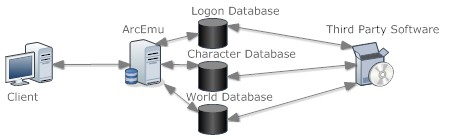
\includegraphics[scale = 0.65]{arcemu.jpg}	
\caption{The architecture used by ArcEmu and how its databases can be accessed}
\label{arcdata}
\end{figure}


Once ArcEmu is set up properly, the client can connect to it as if it were the real WoW server. All the data about NPCs, quests, items and so forth is sent to the client by the ArcEmu server. The server also receives data from the client about what actions the character is doing, which is then distributed to any other connected clients. Communication to and from the database is done exclusively by the server, but it is triggered by actions that the client does. Since ArcEmu uses MySQL, the database can be fully accessed without the use of the server. Figure~\ref{arcdata} shows how third party software has access to the databases used by ArcEmu.

Using ArcEmu thus grants full access to the database of an MMORPG, which can then be monitored and analysed to create models of how MMORPGs store and retrieve data. How exactly this is done is discussed in further detail in chapter~\ref{database}.